% !TeX encoding = UTF-8 !TeX spellcheck = en_US
\documentclass[11pt, a4paper]{article}

% The title of the current document to be produced.
\newcommand{\doctitle}{Assignment \#1}
\newcommand{\assignments}{\bluetext{\textbf{Assignment:}}}
%
\setlength{\unitlength}{1in}
\renewcommand{\arraystretch}{2}
\setlength{\columnsep}{2cm}

\newcommand\dunderline[3][-1pt]{{%
  \sbox0{#3}%
  \ooalign{\copy0\cr\rule[\dimexpr#1-#2\relax]{\wd0}{#2}}}}

\usepackage[sfdefault]{atkinson}
\usepackage[T1]{fontenc}

\def\code#1{\bluetext{\texttt{#1}}}


%------------------------------------------------------------
% Import commands for both teacher and course information.  | NOTE: Change your
% teacher and course info in these files. |
%------>------>------>------>------>------>------>------>-->|
%
%------------------------------------------------------------
%-- Import packages and custom command definitons.          |
%------>------>------>------>------>------>------>------>-->|
%% ==================================
%% ===== Teacher info             ===
%% ==================================
%%
\newcommand{\instructor}{Katelyn Breivik}
\newcommand{\office}{Wean 8319}
\newcommand{\hours}{3pm on Mondays}
\newcommand{\phone}{}
\newcommand{\college}{}
\newcommand{\email}{kbreivik@andrew.cmu.edu}
\newcommand{\faculty}{}
\newcommand{\department}{Department of Physics}
                              %|
%% ==================================
%% ===== Course-specific commands ===
%% ==================================

%- Instructions: change course info here. 
\newcommand{\semester}{Fall 2023}

\newcommand{\ponderation}{2-4-3 (Theory-Lab-Homework)}
\newcommand{\coursetitle}{Astrophysics of Stars and the Galaxy}
\newcommand{\coursenumber}{[33-467]}
\newcommand{\prerequisite}{33-224, 33-234}
 
\input{../includes/packages-imports}                          %|  
\input{../includes/custom-commands}   
%
%---> Genereate & inject metadata                           |
\input{../includes/hyperef.doc.info}                          %|
%------------------------------------------------------------

\topmargin -70pt
\begin{document} 

\normalfont

%-------------------------------------------------------------
%-- Make the header of the document                          |
%------>------>------>------>------>------>------>------>--> |
%---------------------------------------------------------------------
%-- The following produces the document header including the title.  |
%---------------------------------------------------------------------

\noindent % <-- need to have this first.

\hfill	
\begin{minipage}{0.60\textwidth}%
	\raggedleft%
	{\Large \textsc{\doctitle}\par}
	\doublerule 
\end{minipage}%
\vspace{0.9cm}

  
%-------------------------------------------------------------
%-- Problem # 1                                              |
%------>------>------>------>------>------>------>------>--> |
\noindent \dunderline{1.0pt}{\textbf{Problem \#1: Installing Python and Python
packages}}

\noindent Throughout this course, you'll regularly use Python to perform
calculations, analyze data, and make figures to support conclusions you draw. In
order to do this, you'll need to install a minimum set of packages if you don't
already have them. First, make sure you have a working Python installation. My
preferred method is using
\href{https://docs.conda.io/en/latest/miniconda.html}{miniconda} with Python
version 3.10 which is a lightweight Python package manager. You are welcome to
use other package managers if you have a preference!
\vspace{2pt}

\noindent Once you have Python installed, there are a few packages that will
prove to be very useful! Please install at a minimum the Python packages listed
below. Many will have a conda installation available but it's not gauranteed.
You can check to see whether a package is available using the
\href{https://docs.conda.io/projects/conda/en/latest/commands/search.html}{conda
search function}.

\begin{itemize}[itemsep=15pt,parsep=3pt,topsep=3pt,partopsep=8pt]
  \item[]
    \centering
      \renewcommand{\arraystretch}{1.5} % this reduces the vertical spacing
      %between rows    
      \begin{tabular}{ccccc}
        \hline
          numpy & matplotlib & astropy & jupyterlab & astroquery  \\                         
        \hline
      \end{tabular}
\end{itemize}

\vspace{20pt}


\noindent \dunderline{1.0pt}{\textbf{Problem \#2: Accessing astronomical data
from public databases}} 

\noindent One of the most powerful datasets in astronomy is the latest (third)
release from the Gaia satellite. This is partially the case because the data is
public and thus free to use for any astronomical research. One of the easiest
ways to access Gaia data is through the
\href{https://gea.esac.esa.int/archive/}{Gaia ESA Archive}. In the top of the
archive webpage, there are tabs that you can use to perform different searches.
Click on the ``SEARCH'' tab to access the standard search form. 

\begin{figure}[h!]
  \centering
  
\includegraphics[width=15cm]{images/Gaia_ESA_Archive_home.png}
\end{figure}

\noindent \dunderline{1.0pt}{\textbf{Problem \#2a: Searching for individual
sources}}

\noindent Some stars are bright enough that they have been known of since
ancient times because we can see them with our eyes. Because of this, they have
names like Beta Pictoris instead of phone numbers like most modern stars (e.g.
Gaia DR3 4373465352415301632). You can search for both kinds of stars
individually by name in the ``SINGLE OBJECT'' tab. For both Beta Pictorus and
Gaia DR3 4373465352415301632, gather the mean values for the parallax, apparent
brightness in Gaia's G filter, and the mean effective temperature and report
them as your answer. 
\vspace{4pt}

\noindent \dunderline{1.0pt}{\textbf{Problem \#2b: Using bolometric
corrections}}

\noindent Using the Bolometric correction equation $BC_{\rm{G}} =
M_{\rm{bolometric}} - M_{\rm{G}}$ and the following bolometric correction values
for Beta Pictoris and Gaia DR3 4373465352415301632, calculate the apparent
bolometric magnitude for each star. Based on the effective temperatures, why is
Beta Pic's bolometric correction larger? What does this tell us about the Gaia G
filter?

\begin{itemize}[itemsep=15pt,parsep=3pt,topsep=3pt,partopsep=8pt]
  \item[]
    \centering
      \renewcommand{\arraystretch}{1.5} % this reduces the vertical spacing
      %between rows    
      \begin{tabular}{rc}
        \hline
          Beta Pictoris: & $BC_{G} = 0.0172$  \\ 
          Gaia DR3 4373465352415301632: & $BC_{G} = 0.0035$ \\                         
        \hline
      \end{tabular}
\end{itemize}
\vspace{4pt}

\noindent \dunderline{1.0pt}{\textbf{Problem \#2c: Calculating bolometric
luminosities}}

\noindent In order to calculate the bolometric luminosity, we need to first
calculate the \emph{absolute magnitude} using the distance modulus :
$M_{\rm{abs}} = M_{\rm{app}} - 5 \log_{10}(d / 10 \rm{pc})$. This requires the
distance, which can be estimated from the parallax. 
\vspace{2pt}

\noindent First estimate the absolute bolometric magnitude of each star, using
the estimated distance. Then, using the absolute bolometric magnitude of the
Sun, calculate the bolometric luminosity of both Beta Pictoris and Gaia DR3
4373465352415301632. 

\vspace{4pt}

\noindent \dunderline{1.0pt}{\textbf{Problem \#2d: Using the Stefan-Boltzmann
Equation to infer stellar radii}}

\noindent Now that we have the bolometric luminosity of each star, we can use
the measured effective temperature and the Stefan-Bolztmann Equation to infer
the radius of each star. Calculate the radius of both Beta Pictoris and Gaia DR3
4373465352415301632. How do they compare to the Sun's radius? 
\vspace{4pt}

\noindent \dunderline{1.0pt}{\textbf{Problem \#2e: Using the Main-Sequence
Mass--Luminosity relation to infer stellar masses}}

\noindent The Mass--Luminosity relation allows us to estimate the masses of
main-sequence stars by comparing their bolometric luminosities to the bolometric
luminosity of the Sun. Use the M--L relation to estimate the mass of both Beta
Pictoris and Gaia DR3 4373465352415301632. Models using high-resolution spectra
of both stars have been used to perform fits to the masses of each star which
are listed below. How do the M--L relation estimates compare? Compute the
percentage difference between the spectral fits and the M--L estimates.

\begin{itemize}[itemsep=15pt,parsep=3pt,topsep=3pt,partopsep=8pt]
  \item[]
    \centering
      \renewcommand{\arraystretch}{1.5} % this reduces the vertical spacing
      %between rows    
      \begin{tabular}{rc}
        \hline
          Beta Pictoris: & $M = 1.75\,\rm{M_{\odot}}$  \\ 
          Gaia DR3 4373465352415301632: & $M = 0.93\,\rm{M_{\odot}}$ \\                         
        \hline
      \end{tabular}
\end{itemize}
\vspace{4pt}


\vspace{20pt}

\noindent \dunderline{1.0pt}{\textbf{Problem \#3: Downloading astronomical data
from ADQL}}

\noindent If we are instead interested in accessing data from a
\emph{population} of stars, it is not efficient to use individual searches for
each star. The Astronomical Data Query Language (ADQL) is a language similar to
SQL that allows users to search large astronical databases to select
subpopulations of interest. Gaia DR3 contains almost \emph{2 billion} sources
with photometric measurements. This means that we should not try to download the
entire dataset (it will 100\% crash your laptop!).\\

\vspace{4pt}
\noindent \dunderline{1.0pt}{\textbf{Problem \#3a: ADQL with \code{astroquery}}}


\noindent The astroquery Python package provides an interface to the Gaia
database so that you can query data directly using ADQL. This interface is
extremely powerful and thus has a \emph{large} amount of
\href{https://astroquery.readthedocs.io/en/latest/gaia/gaia.html}{documentation}.
For now, let's use the following astroquery syntax to select a subset of $1000$
stars with well-measured parallaxes:

\begin{figure}[h!]
  \centering
  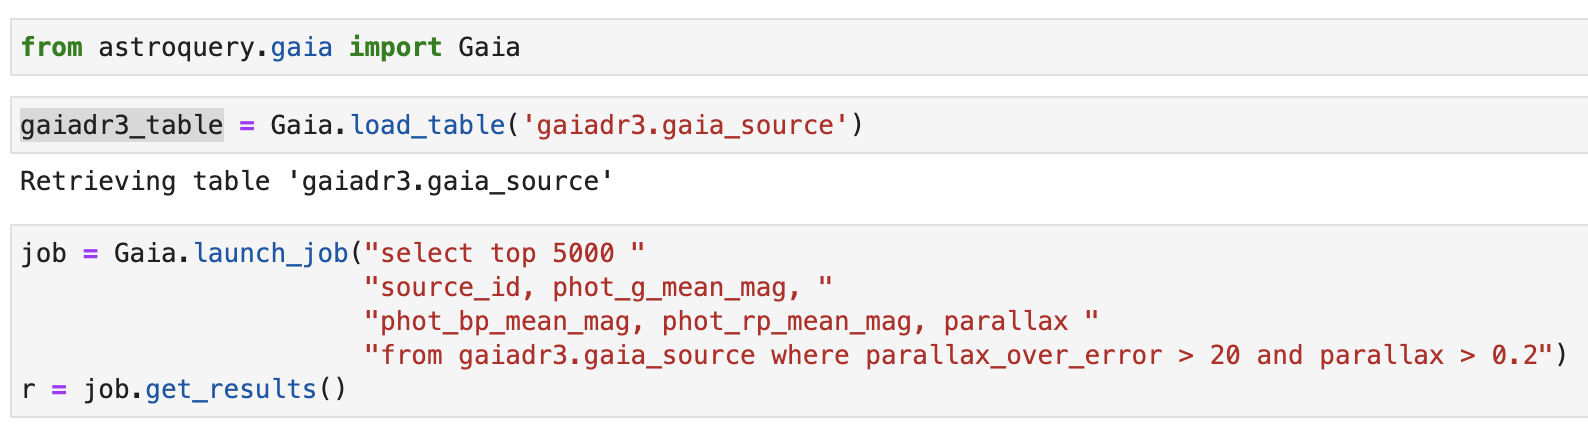
\includegraphics[width=15cm]{images/first_ADQL.png}
\end{figure}

\noindent You should supply the same query by opening a jupyterlab environment
and repeating the same import and query as above. Try printing the results table
\code{r}, which shows each star as a separate row. How does the requirement for
parallax > 0.2 mas influence the distance of the stars in our table?

\vspace{2pt}
\noindent Notice that \code{astroquery} returns a table; this is an
\code{astropy} table which allows you to store \emph{units} in addition to
values for each star. Fields with units are called
\href{https://docs.astropy.org/en/stable/units/}{quantities} and can be
manipulated with the \code{astropy.units} class. 

\vspace{4pt}
\noindent \dunderline{1.0pt}{\textbf{Problem \#3b: Plotting a color-magnitude
diagram (CMD)}}

\noindent Using the \code{matplotlib} package, plot a scatter plot that shows
the color-magnitude diagram which contains the apparent G magnitude on the y
axis and the BP - RP magnitude on the x axis for each source. Be sure to label
each axis!

\noindent If you are unfamiliar with \code{matplotlib}, the best way to learn is
often a google search with "matplotlib" appended. For example, for this figure,
you could search: "matplotlib scatter plot" and "matplotlib xlabel". You may
also find the
\href{https://matplotlib.org/stable/tutorials/introductory/pyplot.html}{pyplot
tutorial} helpful!


\vspace{4pt}
\noindent \dunderline{1.0pt}{\textbf{Problem \#3c: Converting from parallax to
distance with equivalencies in \code{astropy.units}}}\

\noindent Now that we have a column with parallax, we can calculate the distance
assuming that all motion on the sky for each source is due to parallax. The
easiest way to do this is through
\href{https://docs.astropy.org/en/stable/units/equivalencies.html#how-to-convert-parallax-to-distance}{equivalencies}.
In order to use equivalencies, you'll need to import the units class as\
{\center \code{import astropy.units as u}} 
\vspace{4pt}

\noindent You should convert the parallax to distance and store the distance
values in a new column in your \code{r} results table as\

{\center \code{r['distance'] = r['parallax'].to(u.pc,
equivalencies=u.parallax())}}\\

\vspace{4pt}
\noindent \dunderline{1.0pt}{\textbf{Problem \#3d: Creating an absolute CMD}}\

\noindent Using the distance column and the apparent magnitude columns, create
\emph{absolute} G, BP, and RP columns in your \code{r} results table. You can do
this using the distance modulus calculation you did above in question 2.
\vspace{2pt}
\noindent Now plot the color-magnitude diagram, but with the \emph{absolute} G
and BP-RP values. What do you notice has changed? Finally, remake the figure,
but change the y-axis to range from high G to low G (upside down). This is an
absolute color-magnitude diagram which contains stars at different evolutionary
phases. 

\end{document} 
